
\vspace{-8mm}
\begin{figure}[!ht]
     \centering
     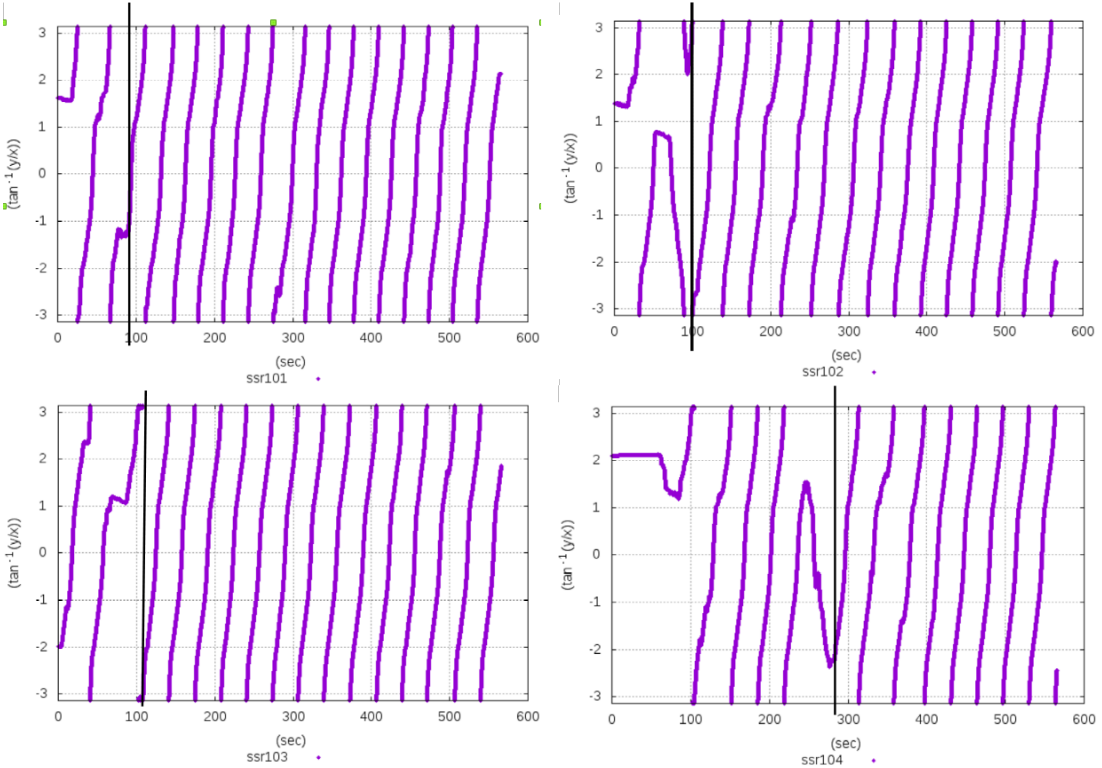
\includegraphics[width=1.0\linewidth]{ssr4_1.jpg}
\end{figure}

\vspace{-8mm}
\begin{figure}[!ht]
     \centering
     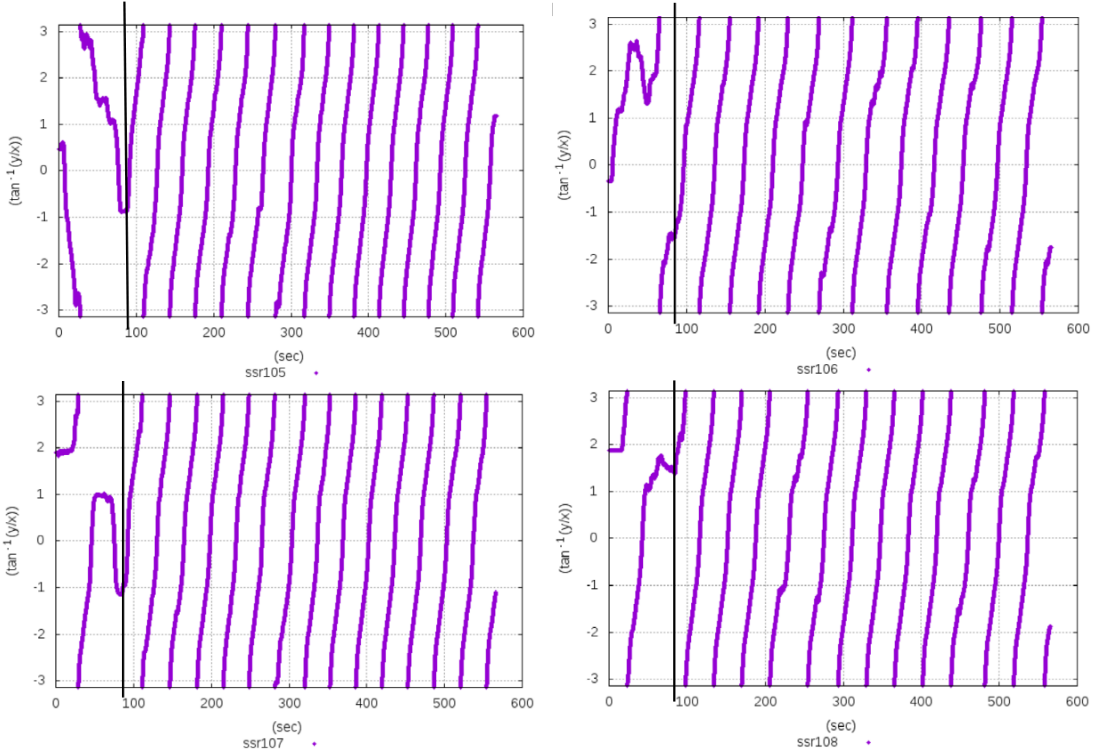
\includegraphics[width=1.0\linewidth]{ssr4_2.jpg}
     \caption{コース中心から見たロボットの角度$\theta$の時間変化}
\end{figure}

図7は各ロボットの$\theta$(図5)と時間の関係図である,横軸は時間(単位:$秒$),縦軸は角度$\theta$である.$T_{\rm sd}$とは全てのロボットが方向転換せず,同じ向きで走る状態になる時間である,図7中の黒い線はロボットが方向転換しなくなるまでの時間,その中で一番長いものを$T_{\rm sd}$とする.




